\documentclass[a4paper,11pt]{article}

\usepackage[pdftex]{graphicx}
\usepackage[pdftex,breaklinks=true,colorlinks=true,linkcolor=black,filecolor=blue,urlcolor=blue]{hyperref}
\usepackage{color}
\usepackage[paper=a4paper,hmargin=3cm,vmargin=4cm]{geometry}
\usepackage{lscape}
\usepackage{amsmath}
\usepackage{listings}
\usepackage{fancyhdr}
\usepackage{subfig}
\usepackage{pdflscape}

% Paragraph style
\setlength\parindent{0in}
\setlength\parskip{0.1in}

% URL style
\def\UrlFont{\small\tt}

\lstset{breaklines=true,basicstyle=\small,tabsize=3,numbers=left,numberstyle=\tiny,numbersep=5pt,emptylines=1}

% Setup fancy headings - copied from lshort
\pagestyle{fancy}
% with this we ensure that the chapter and section
% headings are in lowercase.
\renewcommand{\sectionmark}[1]{%
        \markright{\thesection\ #1}}
\fancyhf{} % delete current header and footer
\fancyhead[LE,RO]{\bfseries\thepage}
\fancyhead[LO]{\bfseries\rightmark}
\fancyhead[RE]{\bfseries\leftmark}
\renewcommand{\headrulewidth}{0.5pt}
\renewcommand{\footrulewidth}{0pt}
\addtolength{\headheight}{0.5pt} % space for the rule
\fancypagestyle{plain}{%
   \fancyhead{} % get rid of headers on plain pages
   \renewcommand{\headrulewidth}{0pt} % and the line
}

\newcounter{savedcounter}

%opening
\title{COMP6026 Assignment 3 \\
Coevolving an Ideal Tetris Trainer}
\author{David Sansome $<$ds505$>$}

\begin{document}
\bibliographystyle{plain}

\maketitle

\begin{abstract}
  It can sometimes be computationally very expensive to reliably evaluate the
  fitness of an individual when its success depends on sequences of random
  events.
  It becomes necessary to evaluate the individual a number of times so that an
  average can be taken and used as the individual's overall fitness.
  
  This report attempts to evolve an ideal sequence of Tetris pieces that can be
  used as a fair test when evaluating the fitness of a Tetris player.
  Using this one ideal sequence instead of a series of random sequences will
  reduce the computation time required to evolve better Tetris players.
  
  Our results show that coevolving Tetris players against Tetramino sequences
  can produce a small improvement in the fitness of the resulting players, but
  further investigation is be required to determine whether this small change
  is just a statistical anomaly.
\end{abstract}

\clearpage
\tableofcontents

\section{Technical Improvements}

\subsection{Tetris players}
\label{players}

The first part of this assignment described an algorithm to evolve a Tetris
player.
Each individual player in the population used a different board-rating function
to choose the best move to make at each stage of the game.
The player's decision was based on six criteria:

\begin{enumerate}
  \item \emph{Pile Height}: The total height of the Tetris board, measured from
      the bottom of the board to the highest occupied cell.
  \item \emph{Holes}: The number of unoccupied cells that have at least one
      occupied cell above them.
  \item \emph{Connected Holes}: Same as \emph{Holes}, except vertically
      connected unoccupied cells only count as one connected hole.
  \item \emph{Removed Lines}: The number of lines that were cleared in the last
      step to get to the current board.
  \item \emph{Altitude Difference}: The difference between the highest occupied
      cell and the lowest free cell that is directly reachable from the top.
  \item \emph{Maximum Well Depth}: The depth of the deepest well on the board.
      A well is a vertical group of unoccupied cells with a width of one,
      reachable from the top and with other filled cells on both sides.
  \setcounter{savedcounter}{\theenumi}
\end{enumerate}

This assignment extends the board-rating function by adding the additional six
criteria used by Mandl \cite{Mandl2005}:

\begin{enumerate}
  \setcounter{enumi}{\thesavedcounter}
  \item \emph{Sum of all Wells}: Sum of the depths of all the wells on the board.
  \item \emph{Landing Height}: The height at which the last Tetramino was placed.
  \item \emph{Blocks}: The total number of occupied cells currently on the board.
  \item \emph{Weighted Blocks}: Same as \emph{Blocks} above, but each occupied
      cell at height $n$ from the bottom of the board counts for $n$.
  \item \emph{Row Transitions}: The sum of all horizontal occupied/unoccupied
      transitions across the board.
      The area outside the board counts as occupied.
  \item \emph{Column Transitions}: The sum of all vertical occupied/unoccupied
      transitions across the board.
      The area above the board counts as unoccupied, and the area below the
      board counts as occupied.
\end{enumerate}

Two additional board rating functions were also implemented.
The previous assignment exclusively used a linear rating function $R_l(b)$
shown in Equation \ref{LinearRating} below, but here we have added the two
other rating functions described in Mandl's paper.
These are the exponential function $R_e(b)$ and the exponential-displacement
function $R_d(b)$.


\begin{equation}
\label{LinearRating}
  R_l(b) = \sum^6_{i=1} w_ir_i(b)
\end{equation}

\begin{equation}
\label{ExponentialRating}
  R_e(b) = \sum^6_{i=1} w_ir_i(b)^{e_i}
\end{equation}

\begin{equation}
\label{DisplacementRating}
  R_d(b) = \sum^6_{i=1} w_i \lvert r_i(b) - d_i \rvert ^{e_i}
\end{equation}

These functions add some more genes to the individual - the set of exponents
$e$ and the set of displacements $d$.
Both these sets contain real-valued numbers and are the same size as the set of
weights $w$ used in the original individual.
When initially seeding the player population with individuals we chose integer
values for the weights randomly from the range $-1000 \cdots 1000$.
Similarly we choose random real numbers for the exponents from the range
$-2.0 \cdots 2.0$, and displacements from $-10.0 \cdots 10.0$.

\subsection{Random numbers}

The previous assignment generated pseudo-random numbers by calling the
\emph{rand\_r()} C library function.
The implementation of \emph{rand\_r()} suggested in the C99 specification
\cite{C99} uses a 16-bit seed and is well known for its poor statistical
properties and small cycle especially in the low-order bits.
The implementation in the GNU C library is slightly better, as it uses a 32-bit
seed, but still suffers from the same problems.

We make use of random numbers in almost every part of this project, and the
reliability of our results depends on these numbers being unpredictable and with
a very high cycle.
Because we generate so many random numbers it is also advantageous for the
psuedo-random number generator to be fast (\emph{rand\_r()} is very slow).

The Mersenne Twister \cite{matsumoto1998mersenne} generator has a cycle of
$2^{19937}$ (compared to \emph{rand\_r()}'s $2^{32}$) and is generally regarded as
being the most suitable general-purpose generator.
However we chose to use a Lagged Fibonacci \cite{brent1992uniform} generator
with parameters $p=607$, $q=273$.
This generator has a faster execution time than Mersenne Twister and repeats in
a cycle of $2^{32000}$, however this comes at the cost of increased state (4.7kb
instead of 2.5kb).

The implementations from the Boost Random Number
Library\footnote{\url{http://www.boost.org}} were used.

\subsection{Population diversity}

In a long running evolution it is possible for the individuals to become
genetically very similar to each other as the least fit ones are eliminated and
the fittest reproduce amongst themselves.
Diversity in the population is required to ensure that the algorithm does not
``home in'' on a local minimum without any chance of jumping away.

We would like to measure the diversity of the genes within chromosomes (weights,
exponents and displacements) in our Tetris player population.
This measure can then be used to decide whether it is necessary to introduce
fresh, random individuals into the population.

Nsakanda et al.\ \cite{nsakanda2007ensuring} provide an overview of the common
ways of measuring population diversity in genetic algorithms, including the
entropy measure suggested by Grenfenstette \cite{grefenstette1987incorporating}.
Burke et al.\ \cite{burke2003advanced} compare a selection of more advanced
population diversity measures.

For this project we decided to settle on a more straightforward way of measuring
diversity: standard deviation.
If we take the value of the $j^\textrm{th}$ gene from individual $i$ to be
$g_{ij}$, then the diversity of the population can be measured as:

\begin{equation}
  D = \sum_{i=1}^{n_p} \frac{\sqrt{\frac{\sum_{j=1}^{n_g} (g_{ij} - \overline{g_i})^2 }{n_g}} }{n_p}
\end{equation}

Where $n_p$ is the number of individuals in the population, and $n_g$ is the
number of genes composing each individual.
The diversity was of course measured seperately for each chromosome as the
genes in different chromosomes have different precisions and ranges and would be
incompatible when measured together.

\section{The Problem}

\subsection{Overview}

The inherent difficulty in finding a good Tetris player is that games of
Tetris are based around a random sequence of Tetraminos - a player that is
successful in one game of Tetris may not be so successful in another game with
a different sequence.
The original assignment tackled this problem by allowing each player to play
12 games and taking the average number of blocks placed over all the games as
the player's fitness.
While this does increase our confidence in the results, it is also
computationally quite expensive.
We would like to be able to find a single non-random sequence of Tetraminos
that can be used to train our algorithm.

The question therefore, is:

\begin{quote}
  Can we evolve a sequence of tetraminos that trains players to be good on a
  variety of random sequences?
\end{quote}

Using coevolution to evolve the tetramino sequence seems like an appropriate
strategy.
Coevolution has been used in the literature to improve the performance of
players in other similar games, including Chinese Chess
\cite{ong2007discovering}, Checkers \cite{chellapilla1999evolving} and
Othello \cite{moriarty1995discovering}.
These games all require two players, and so the algorithms use competitive
coevolution to play two players off against each other - the winner is given a
higher fitness and the loser a lower fitness.
Tetris is a single player game so we cannot use the same approach, instead we
shall introduce a second population of Tetramino sequences and assign fitness
values to them based on their similarity to a good ``random'' sequence.

\subsection{The new individual}

There are a number of different representations we can use for a sequence of
Tetraminos:

\label{individualtype}
\begin{enumerate}
  \item \emph{Random seed} - the individual would hold a single gene containing
      the seed for a deterministic pseudo-random number generator.
      Each generated number would represent a single Tetramino dropped onto the
      board.
      While this would require the smallest possible storage space, it would be
      impossible to evolve or mutate, as the smallest change to the seed would
      result in an entirely different sequence of random numbers.
  \item \emph{Small repeating sequence} - the individual would contain a short
      fixed-size sequence of Tetraminos which would be ``rewound'' and used
      again when they had been exhausted.
      This representation lends itself well to manipulation by crossover and
      mutation operators, but could lead to biased games of Tetris.
      A strategy that effectively cleared the sequence the first time it
      appeared would be able to do exactly the same thing next time the
      sequence was produced, and games would be artifically lengthened.
      This problem is the same as that of a psuedo-random number generator with
      a short cycle.
  \item \emph{Exhaustive sequence} - the individual would contain an infinite
      sequence of Tetraminos.
      Obviously we cannot really store an infinite sequence, so this would be
      identical to a very large \emph{small repeating sequence} that didn't
      repeat.
      Storing 1,000,000 tetramino values takes approximately 1MB of memory and
      still has acceptable performance when mutating and reproducing.
  \item \emph{Markov chain} - each \emph{state} in the Markov chain would
      represent the emission of one Tetramino, and the probabilities of moving
      between states would make up the individual's genes.
      High order Markov chains would likely give more structure to the
      Tetramino sequences.
      Hoogeboom and Kosters \cite{hoogeboom2004tetris} use finite state
      automata to generate sequences of Tetraminos in their research on
      decidability.
\end{enumerate}

We chose to use the \emph{exhaustive sequence} representation as it is
straightforward and can be easily evolved.
The mutation operator has a probability $p$ of replacing a Tetramino in the
sequence with a new randomly selected Tetramino.
Two crossover operators were evaluated - the uniform crossover operator would
randomly select genes from the two parents with equal probability.
The one-point crossover operator would randomly select a point in the Tetramino
sequence and take genes on one side of that point from the first parent and
genes on the other side from the second parent.

\subsection{Fitness function}

The goal of this evolution is to find a Tetramino sequence that, when used by
a given player, leads to similar performance as a series of random sequences.

During each generation we pair each player up with a Tetramino sequence and let
them play one game.
The number of blocks that a player $P$ places given a game using sequence $S$
is denoted as $f(P, S)$.
Like in the previous assignment, this value is also taken to be the fitness of
that player in its population:

\begin{equation}
  f(P_i) = f(P_i, S_i)
\end{equation}

We now take each of these players and make them play $N$ new games against
random sequences of Tetraminos - $S_r$.
Again we record the number of blocks placed during each of these additional
games, but this time we compare this value with the number of blocks that were
placed in the original game.
This tells us how similar the sequence is to a random sequence, and how fair a
measure it is of an individual player's performance.

The average distance from the sequence $S_i$ to these random games is denoted
by $D_i$ and calculated as follows:

\begin {equation}
  D_i = \sum_{j=1}^{N} \left| f\left( P_i, S_i\right) - f\left( P_i, S_r \right) \right|
\end{equation}

We then have to normalise this value for number of games played, as well as the
original fitness (or else bad sequences that happened to be played by fitter
players would end up with higher fitnesses than good sequences played by bad
players).
We also scale the range of values so they lie within the range $[0, 4000]$.
This was chosen somewhat arbitrarily, but it is the same order of magnitude
as our other fitness values.

\begin{equation}
  f(S_i) = 1000 \left( \max 0, 2 - \frac{D_i}{ N f\left( P_i, S_i\right) } \right)^2
\end {equation}

Psuedo-code for this algorithm is shown in Listing \ref{psuedocode} below.


\begin{lstlisting}[firstnumber=1,language=c,morekeywords={until,foreach,in},frame=single,mathescape=true,caption={Pseudo-code of the algorithm used to evolve one generation},label={psuedocode},float=[htb]]
for 0 $\leq$ i $<$ population.size
  // One member from the player population plays a game with one member
  // from the sequence population.
  blocks_placed = PlayGame(player[i], sequence[i])
  player[i].fitness = blocks_placed
  
  // The same player now plays games against random sequences
  random_fitness = 0
  for 0 $\leq$ game $<$ kNumberOfGames
    random_fitness += abs(blocks_placed - PlayGame(player[i], RandomSequence()))
  random_fitness /= kNumberOfGames
  
  // The sequence's fitness is derived from how similar it was
  // to the random games
  sequence[i].fitness = Normalise(random_fitness)
\end{lstlisting}

\section{Results}

\subsection{Technical improvements}

The technical modifications to the Tetris players led to the biggest
improvements in fitness.
By the end of the previous assignment the very best Tetris players could place
around 2-3 thousand blocks over the course of a game.
After adding the remaining six board rating criteria discussed in Section
\ref{players} the performance increased by an order of magnitude, and the best
players were now able to place 20,000 blocks easily, sometimes reaching 50,000
and above.

Figure \ref{LinearNoCoev} shows how the mean fitness of the player population
increases over time.

\begin{figure}[h]
  \label{LinearNoCoev}
  \centering
  \includegraphics[width=13cm]{results/linear-no-coev.png}
  \caption{Mean player fitness over time from 10 different executions.}
\end{figure}

Adding in the exponential rating function has not been as useful, and actually
gives worse performance than the linear rating function.
This is possibly due to larger search space - it is more difficult for the
algorithm to find a suitable set of parameters.

A comparison of the changes is given in the table below.

\begin{center}
  \begin{tabular}{l l l l}
    \hline
     & Max & Mean & Lowest \\
    \hline
    First six board criteria & 2145 & 599 & 128 \\
    All twelve board criteria & 58382 & 4605 & 108 \\
    Exponential rating function & 16330 & 2332 & 116 \\
    
  \end{tabular}
\end{center}

\subsection{Population diversity}

Measuring the standard deviation of player chromosomes has revealed some
interesting results.
While the diversity of the \emph{weights} chromosome decreases initially, it
always seems to level off and sometimes increase again at around the
20-generation point.
Decreasing diversity is of course expected as the population gains fitness
because all the initial random low-fitness players are being eliminated.
However the increase again is curious, and suggests that our mutation rate is
sufficient (or even too high?) to maintain diversity in the population.

\newcommand{\smallgraphwidth}{7cm}
\begin{figure}[h]
  \centering
  \subfloat[Weights]{\label{stddev-w}\includegraphics[width=\smallgraphwidth]{results/linear-stddev.png}}
  \qquad
  \subfloat[Exponents]{\label{stddev-e}\includegraphics[width=\smallgraphwidth]{results/exponential-stddev.png}}

  \caption{Comparing the standard deviation of chromosome values to player
      fitness.
      The blue line is player fitness and the red line is standard deviation
      of the measured chromosome.}
  \label{stddev}
\end{figure}

The \emph{exponent} chromosome loses diversity very rapidly, usually ending up
having a standard deviation of around 0.3.
Maybe this means a higher mutation rate is required for the exponent values, or
maybe the diversity needs to be maintained by adding new random individuals
occasionally.

\subsection{Coevolution}

Figure \ref{LinearCoev} below shows the difference in performance between games
in which the player population plays an evolving population of Tetramino
sequences, and games in which the player population plays random sequences.
We would expect individuals playing with the evolving sequences to get better
than their random-playing counterparts over time as the sequences evolve to
become more ``fair''.

This does indeed happen, although the change in performance is small.
Players playing against the evolving sequences finish with fitnesses between
3400 and 5201, and players playing random sequences finish slightly lower
between 2200 and 4600.

\clearpage

\begin{figure}[h]
  \label{LinearCoev}
  \centering
  \includegraphics[width=13cm]{results/linear-coev-vs-no-coev.png}
  \caption{Comparison of player performance with and without coevolution.
      Feint lines show the performance over time of 10 runs - five (blue) in which
      the player population played against an evolving population of Tetramino
      sequences, and five (red) in which the players played against random
      sequences.
      Strong straight lines are trendlines for the average of the five games.}
\end{figure}

It is quite difficult to draw conclusions from these results, as the difference
in performance can just as easily be explained by random chance - it is
possible that the players in the five runs against evolving sequences just
happened to be more lucky.

To be sure that coevolution actually helped improve the player performance we
would need to run more tests each lasting for more generations.
Also it would be useful to try evolving the sequence for longer, artificially
slowing the evolution of the players by introducing new random players into the
population or increasing their mutation rate.
It would be interesting to see how a fresh population of players coped with a
population of sequences that had already been evolved.

Sadly there was not enough time to try any of these extra tests.

\section{Future Work}

The representation of Tetramino sequences as evolvable units is currently quite
basic, and there are a number of changes that could be made to make them better
at finding the perfect training sequence:

\begin{enumerate}
  \item Uniform crossover and one-point crossover are currently used when
      forming a new sequence individual.
      The fixed sequence representation detailed in Section \ref{individualtype}
      seems perfect for a more \textbf{sophisticated crossover operator}
      that takes small (10-20) Tetramino sequences from each parent.
      Adjacent genes in the Tetramino sequence are naturally related, as
      success in Tetris is dependent on having complimentary Tetraminos
      appearing sequentially.
  \item The idea of using a \textbf{Markov chain} representation for the
      sequence individuals mentioned in Section \ref{individualtype} was never
      attempted.
      It would be interesting to try this, as perhaps different strategies
      would develop if there was some pattern to the Tetraminos being dropped
      as opposed to their selection being seemingly random.
      The new mutation operator would change the state transition probabilities
      of the Markov chain, and would therefore have more of a direct and
      deterministic change on the pattern than the current operator that simply
      changes the occasional block in the sequence.
\end{enumerate}

\clearpage
\bibliography{../COMP6026}

\appendix
\clearpage
\section{Sequence visualisation}

\begin{figure}[h]
  \label{Sequence}
  \centering
  \includegraphics[width=13cm]{results/sequence.png}
\end{figure}

If you render each Tetramino in a sequence as a single coloured
pixel (red is the square, green is the line piece, blue is the squiggly,
etc.) then it looks something like this.
This can be useful as a quick visual check that the sequence is mostly
random.
I tried to use Dieharder\footnote{\url{http://www.phy.duke.edu/~rgb/General/dieharder.php}}
(a random number test suite) to perform various statistical tests on the
generated sequences, but it doesn't seem to work well with small ranges of
values.

\section{Source code}
\begin{center}
 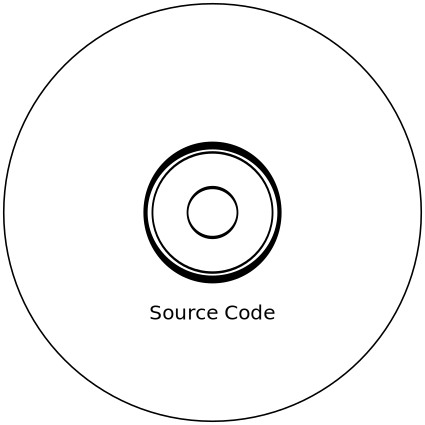
\includegraphics[width=12cm,height=12cm]{cd.png}
\end{center}


\end{document}
